\section{Calculation of Sea Level Pressure}

Over land, surface pressure is dominated by the land surface elevation rather than the position of low pressure centers, fronts, etc. In order to see these features, surface pressure must be converted to sea level pressure, also known as the pressure at sea level (PSL, denoted here by $p_s$), which is the surface pressure we would have if the landmass was not there. There's no single accepted set of assumptions for how this ``subterranean atmosphere'' should behave. What is its lapse rate? How much moisture does it contain? Because PSL is just a diagnostic output for EAMxx, our current implementation just copies what EAMf90 did, which was inherited from an early version of the Community Atmosphere Model. This approach is outlined in Section 3.1B of \cite{Trenberth_et93} but that document isn't very clear so we describe the approach below. 
%Trenberth, K. E., Berry, J. C., & Buja, L. E. (1993). Vertical Interpolation and Truncation of Model-coordinate Data (No. NCAR/TN-396+STR). University Corporation for Atmospheric Research. doi:10.5065/D6HX19NH

%================================
\subsection{Formulation}
%================================

The basic idea is to assume the subterranean atmosphere is free of moisture and has a lapse rate $\Gamma = 6.5$ K km$^{-1}$ unless the atmosphere is too warm or too cold, in which case the lapse rate and the ground temperature are empirically modified to provide more reasonable results (as described later). The hydrostatic equation $\partial p/\partial z = -\rho_\mathrm{air} g$ is integrated from a height of zero (sea level) to the height of the ground to compute sea level pressure. Because the model stores geopotential $\Phi$ rather than geopotential height $z$, we rewrite the hydrostatic equation using $\Phi = gz$ (where $g$ is the gravitational constant). We also use the ideal gas law $\rho_\mathrm{air} = p/(R_d T)$ (where $R_d$ is the gas constant for dry air) to write density in terms of pressure and temperature. Thus our hydrostatic equation is
%-------------------------------------
\begin{equation}
  \frac{\partial p}{\partial \Phi} = \frac{-p}{R_d T}
\label{eq:hydrostat}
\end{equation}
%-------------------------------------
Because lapse rate is assumed linear, the temperature at any $\Phi$ is
%-------------------------------------
\begin{equation}
  T = T_\mathrm{g} + \frac{\Gamma}{g}\left(\Phi_g - \Phi \right)
  \label{eq:T}
\end{equation}
%-------------------------------------
where the subscript $g$ refers to the value of the atmosphere at ground level (i.e. the bottom interface of the lowest atmosphere grid cell). Note that $\Gamma$ is positive in this formulation. For our subterranean atmosphere, $\Phi$ varies between 0 (sea level) and $\Phi_g$, which should be positive except in a few rare depressions like Death Valley. As a result, we expect $T$ to be warmer than $T_g$ most but not all of the time. 

Integrating (\ref{eq:hydrostat}) over the vertical after substituting (\ref{eq:T}) yields:
%-------------------------------------
\begin{equation}
  \int_{p_s}^{p_g} \frac{\partial p}{p} = \int_0^{\Phi_g} \frac{-\partial \Phi}{R_d \left[T_\mathrm{g} + \frac{\Gamma}{g}\left(\Phi_g - \Phi\right)\right]}.
  \label{eq:integral}
\end{equation}
%-------------------------------------
For $\Gamma \ne 0$, this equation can be solved exactly by making the substitution $x = R_d (T_\mathrm{g} + \Gamma/g \left(\Phi_g - \Phi\right) )$, which yields
%-------------------------------------
\begin{equation}
  p_s = p_g \left[ 1+\frac{\Gamma \Phi_g}{g T_g} \right]^{g/(R_d \Gamma)}.
  \label{eq:exact_soln}
\end{equation}
%-------------------------------------
If $\Gamma=0$, the exact solution is
%-------------------------------------
\begin{equation}
  p_s = p_g \exp\left\{\frac{\Phi_g}{R_d T_g}\right\}.
  \label{eq:exact_0gamma}
\end{equation}
%-------------------------------------
Because we will set $\Gamma$ to zero when $_g$ gets too warm, using exact solutions would require conditional execution which is inefficient on GPUs. Also, computing non-integer exponents is expensive. Thus we note that the integrand on the right-hand side of (\ref{eq:integral}) can be written as $A \cdot 1/(1-y) = A \sum_{k=0}^\infty y^k$ for $A=1/(R_d T_g)$ and $y=\Gamma/(g T_g)(\Phi - \Phi_g)$. Because $y$ is always much less than 1, accurate approximations can be made from just the first 3 summands. This leads to
%-------------------------------------
\begin{equation}
  p_s \approx p_g \exp\left\{\beta \left[1 - \frac{\alpha \beta}{2} + \frac{(\alpha \beta)^2}{3} \right] \right\}
  \label{eq:approx_soln}
\end{equation}
%-------------------------------------
for $\alpha=\Gamma R_d/g$ and $\beta=\Phi_g/(R_d T_g)$.

If $T_g<255$ K, (\ref{eq:approx_soln}) is applied with $T_g$ modified according to $\widetilde{T_g} = (255 - T_g)/2$. If $T_g>290.5$ K, a trial sea-level temperature $\widetilde{T_s}$ is computed using (\ref{eq:T}) with $\Phi = 0$ and $\Gamma = 6.5$ K km$^{-1}$. If $\widetilde{T_s}$ is also greater than 290.5 K, $\Gamma$ is set to zero (to prevent temperatures near sea levels from getting even warmer) and $\widetilde{T_g} = (290.5 - T_g)/2$ is used in (\ref{eq:approx_soln}). If $T_g>290.5$ K but $\widetilde{T_s}<290.5$ K, excessive temperatures are prevented by choosing $\Gamma$ such that sea-level temperature just reaches 290.5 K. Note that these crude hacks accomplish their intended goal of avoiding extreme temperatures in a smooth way when $\Phi_g>0$, but may not be appropriate when $\Phi_g<0$. We didn't bother to improve this treatment because accurate $p_s$ isn't a major goal for us and  the current treatment survived without complaint for the last 28 yrs. 

%================================
\subsection{Validation}
%================================

Fig. \ref{fig:exactVSapprox} compares the exact solutions from (\ref{eq:exact_soln}) and (\ref{eq:exact_0gamma}) against the 2nd order Taylor series we use in our calculations and the cruder 1st order approximation. Both approximations agree very well with the exact solutions. In fact, the first-order approximation is probably sufficient for our uses - it is at most 1 mb worse than the 2nd order result in even the most extreme cases. For the $\Gamma=0$ case, both approximations are off by as much as 6 mb, but the 1st order approach isn't any worse than the 2nd order version. 
%----------------------------------------------
\begin{figure}[ht]
\noindent
\centering
\rotatebox{0}{
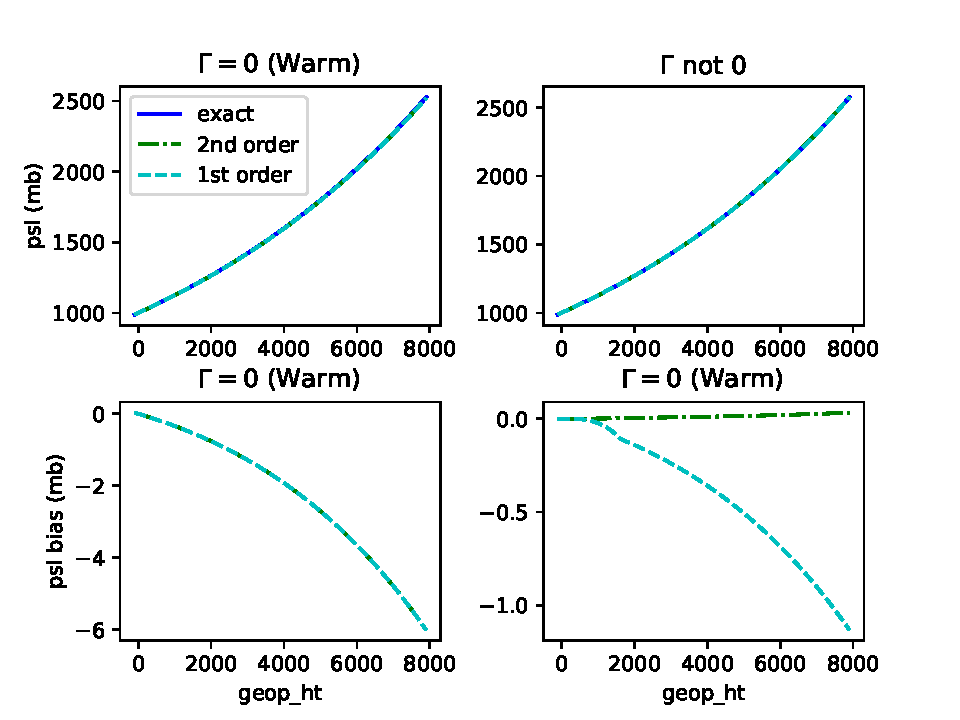
\includegraphics[keepaspectratio=true, width = 4.5in]
{psl_exactVSapprox.pdf}}
\caption{Tests of exact versus approximate $p_s$ calculations. Left panels are warm enough that $\Gamma=0$ ($T_g=292$ K) while right panels use $\Gamma=6.5$ K km$^{-1}$ ($T_g=280$ K). Top panels show actual $p_s$ and bottom panels show bias. Sea level pressures are much too high because $p_g=1000$ mb, but this should be fine for testing purposes. Note that the lowest elevation sampled is -100 m to test behavior when terrain is below sea level.} 
\label{fig:exactVSapprox}
%EXPLANATION:
%/g/g11/caldwep/py/scream/v1/calc_psl.py
\end{figure}
%----------------------------------------------

Fig. \ref{fig:psl_vs_v0} compares $p_s$ from an old F90 simulation against values calculated using our approximate formula. As expected, results look very similar despite using midpoint $T$ as an approximation for $T_g$. Using a first-order rather than 2nd order Taylor series once again has an insignificant effect. 
%----------------------------------------------
\begin{figure}[ht]
\noindent
\centering
\rotatebox{0}{
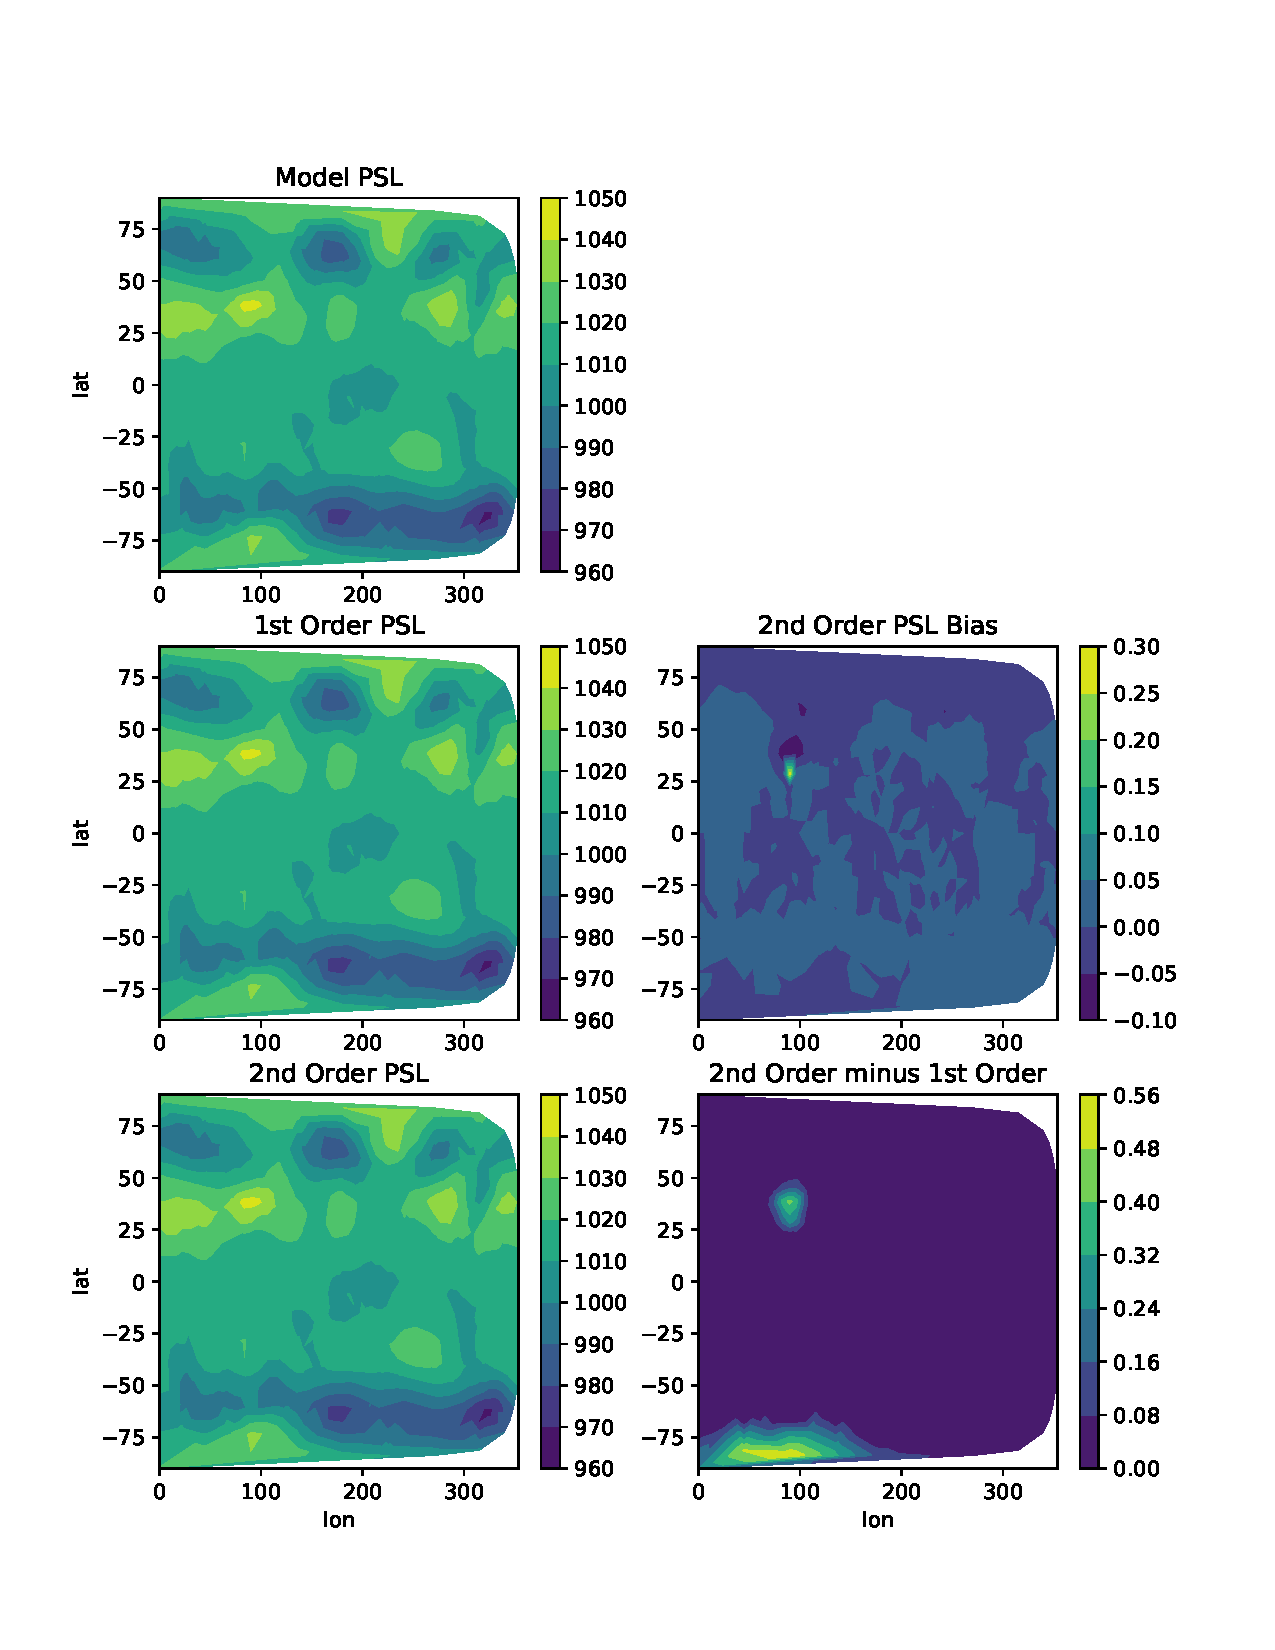
\includegraphics[keepaspectratio=true, width = 5in]
{psl_vs_v0.pdf}}
\caption{Comparison of $p_s$ from an old ne4 F90 model simulation (top left) versus calculation of the same quantity using (\ref{eq:approx_soln}). Panels on the left show $p_s$ and right-hand panels show differences between simulations. Calculated $p_s$ used midpoint rather than surface temperature because the latter wasn't available; this likely accounts for most of the F90 vs new calculation differences we see; despite this imperfection, biases are still acceptably low.} 
\label{fig:psl_vs_v0}
%EXPLANATION:
%/g/g11/caldwep/py/scream/v1/calc_psl.py
\end{figure}
%----------------------------------------------

%================================
\subsection{Unit Tests}
%================================

\begin{enumerate}
\item Is C++ value close to exact solution for very warm conditions where $\Gamma$ should be zero? 
\item Is C++ value close to exact solution for normal conditions where $\Gamma$ should be 6.5 K km$^{-1}$?
\item Is $p_s<p_g$ when $\Phi_ground>0$ (for very cold, moderate, and very warm $T_g$ and a variety of $p_g$ values)?
\item Is $p_s>p_g$ when $\Phi_ground<0$ (for very cold, moderate, and very warm $T_g$ and a variety of $p_g$ values)?
\item Test that modified $T_g$ values for very cold and very warm conditions are applied correctly. Not sure how to do this - should computation of $\widetilde{T_g}$ be its own unit? Or should modified $T_g$ be computed in the unit test itself and stuffed into the exact solution to provide an independent calculation of the expected solution? Or is this too dumb to test?
\end{enumerate}


